\chapter{Negative friction coefficient}\label{chap:negative_coef}

For the final part of this thesis, we concern ourselves with a proof of concept approach for the designing of a negative friction coefficient. From the pilot study (\cref{chap:pilot_study}) we found the two investigated patterns to have a non-linear relationship with sheet strain. By proposing a nanomachine coupling between normal load and strain we investigate the prospects of achieving a negative friction coefficient for these patterns.

\section{Nanomachine coupling}
We do not attempt to simulate the dynamics of any nanomachine desings, but we propose that a coupling could be achieved, for instance by following a design as sketched in \cref{fig:nanomachine}. This could perhaps be achieved by rigging carbon nanotubes in a similar configuration. 

\begin{figure}[H]
  \centering
  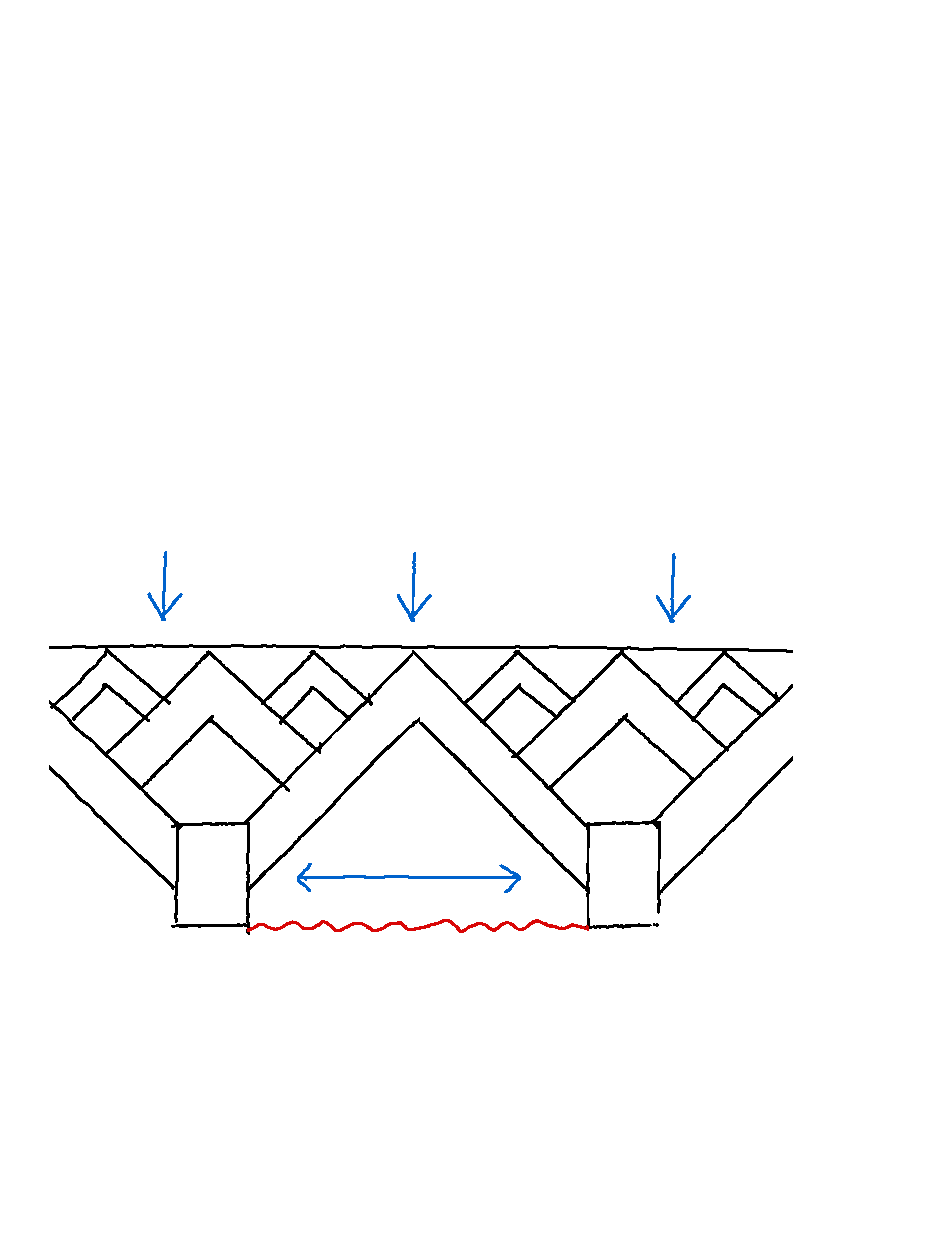
\includegraphics[width=0.5\linewidth]{figures/negative_coefficient/nanomachine.pdf}
  \caption{Working sketch for nanomachine}
  \label{fig:nanomachine}
\end{figure}

We mimic the nanomachine coupling by implementing a load-depending tension force to our \acrshort{MD} simulations. So far, we have kept the pull block spaced by a fixed distance throuhout the simulations, but now we let the pull blocks move relative to eahc other under the influence of a nanomachine tension force between the blocks. The tension force $F_t$ is modeled to be proportional to the normal load $F_t = RF_N$ by a factor $R$ which represents the ratio for the load to strain coupling. We find that a ratio of
$R=6$ will provide the necessary tension for achieving a full strain range (till rupture) within the loading range used so far in our study. We use the Tetrahedron
$(7,5,1)$ and Honeycomb $(2,2,1,5)$ from the pilot study and perform multiple
simulations for different loads. We sample 100 pseudo uniform normal force
values in the $[0, 15]$ nN which corresponds to a tension force of $[0, 90]$ nN. For the Tetrahedron pattern we increase the load by a speed of \SI{0.015}{nN/ps}, but due to a rapid change in the strain for the Honeycomb pattern we reduced the loading speed to \SI{0.0015}{nN/ps} and added additional points to the range of rapidly chaning strain. We compare the results to that from the pilot study \cref{fig:multi_stretch} and consider the strain-tension curve in addition as shown in \cref{fig:negfric}.

% Mention that we had to decrease the ratio for which load increased for the honeycomb.






\begin{figure}[H]
  \centering
  \begin{subfigure}[t]{\textwidth}
      \centering
      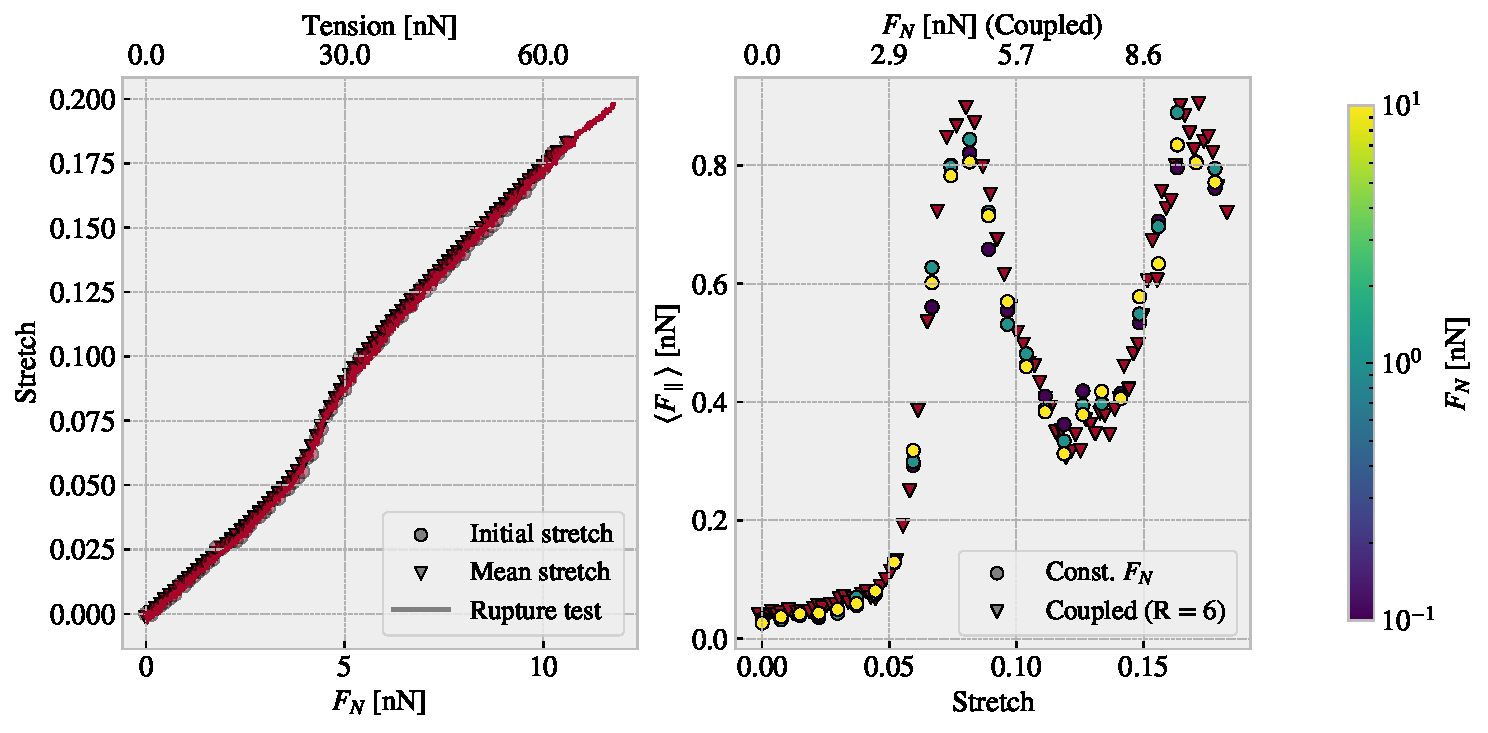
\includegraphics[width=\textwidth]{figures/negative_coefficient/manual_coupling_free_pop7_5_1.pdf}
      \caption{Tetrahedron $(7,5,1)$}
      % \label{fig:}
  \end{subfigure}
  \hfill
  \begin{subfigure}[t]{\textwidth}
    \centering
    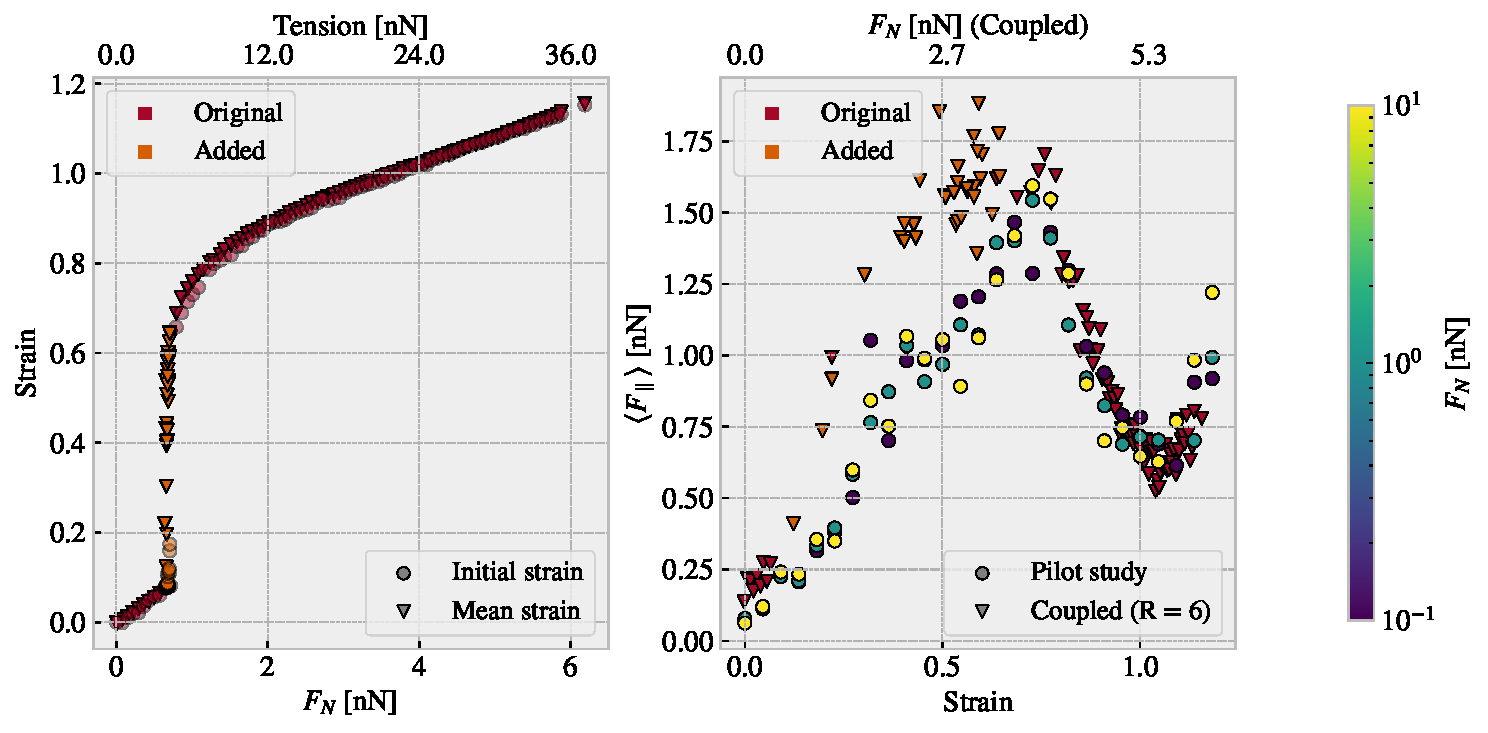
\includegraphics[width=\textwidth]{figures/negative_coefficient/manual_coupling_free_hon2215.pdf}
    \caption{Honeycomb $(2,2,1,5)$}
    % \label{fig:}
  \end{subfigure}
  \hfill
  \caption{Evaluation of the friction response for a coupled system using (a) the Tetrahedron $(7,5,1)$ and (b) Honeycomb $(2,2,1,5)$ pattern.  The pull blocks are allowed to move relative to each other under the influence of a tension force $F_t$ modeled as $F_t = RF_N$ for normal load $F_N$ and a ratio $R=6$. The right panel shows the friction vs.\ stretch curve in comparison to the locked pull block system and constantly defined normal from the pilot study (\cref{fig:multi_stretch}). The left panel shows the strain-tension curve. For the Honeycomb pattern, we added more data points in the region where the strain-tension curve changed rapidly.}
  \label{fig:negfric}
\end{figure}

Generally, we observe from \cref{fig:negfric} that the coupled system follows a
similar trend as seen in the pilot study. Especially the Tetrahedron pattern
aligns well with the comparison data. This first of all shows that the
simultaneous loading and straining of the system does not suppress the
non-linear trend. In both cases, we also notice that the initial and the mean
strain aligns rather well. This indicates that the sliding does not contribute
to a significantly increased tension in the sheet which would otherwise lead an increased strain as well. For the Honeycomb pattern, we find an
interesting trend for the strain-tension curve. At low tension, the curve of the
strain is increasing seemingly linearly with strain, however, a drastic increase
in strain happens at \SI{4.5}{nN} ($F_N = \SI{0.75}{nN}$) transitioning from a
strain of roughly 0.08 to 0.7. Eventually this settles off into a linear trend
before reaching the rupture point. This reflects the reason for decreasing the loading speed and adding more data points to fill this gap in strain. When considering the friction-strain curve we notice that the coupled system results deviates most in the area of rapidly increasing strain. From a closer examination of the simulation frames in \cref{sec:sheet_stretch} we
notice that the strain range covered in this rapid transition aligns rather well
with the unfolding of the honeycomb pattern. More precisely, we find that the
Honeycomb pattern unfolds in segments buckling one at a time after passing a
minimum tension. During the unfolding phase the friction increases, but immediately starts to decrease after being fully unfolded. For further studes we might investigate such transitions in order to get a better understanding of the underlying mechanisms being in play.
